\section{Overview}

The Moving Object Pipeline System has two main responsibilities: the
generation and maintenance of the Moving Object database ({\it i.e..}
the discovery and linking of all observations of each moving object),
and the prediction of known object locations which are sent to the
Alert Pipeline to prevent unneccessary alerts.  To serve these
two functions, MOPS operates in two components, known as ``DayMOPS''
and ``NightMOPS.''

``NightMOPS'' (operating throughout each night) is responsible for
predicting the locations of known Moving Objects in upcoming
images. This is intended solely to help flag known moving objects in
the LSST alert stream.  ``DayMOPS'' (operating after each night's data
is complete, typically in the day) is responsible for discovering new
Moving Objects in newly-acquired data, searching old data for
detections of new objects (`precovery), identifying known moving
objects in newly-acquired data (`attribution') and updating the Moving
Objects database. Note that `attribution' is distinct from
NightMOPS, as attribution can take advantage of additional information
coming from observations throughout the entire night, allowing matches
between new detections and moving objects under larger positional
uncertainties, and also folds this information back into the Moving
Object database. DayMOPS is also responsible for periodically refining
the contents of the Moving Objects database based on the orbits of the
known objects.

The relationship between NightMOPS, DayMOPS, and the neighboring
components of the LSST Data Management system is illustrated in
figure \ref{mopsWithinLsst}.

\begin{figure}[!ht]
\centering
  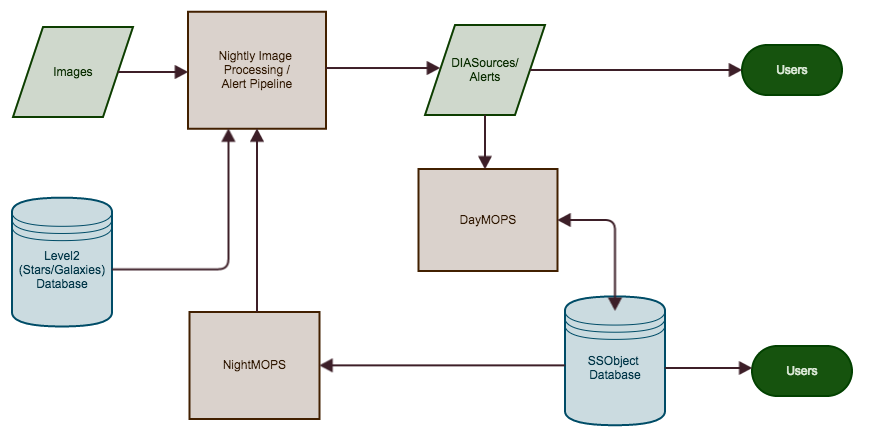
\includegraphics[width=12cm]{illustrations/MOPSinLSST.png}
\caption[Data flow between MOPS and LSST.]{Data flow within LSST, from image acquisition to the Moving
  Object database and Alert generation.  DayMOPS will build and maintain the
  Moving Objects table, NightMOPS will use the Moving Objects table to
  predict positions of known moving objects and
  communicate with the Assocation Pipeline.  }
\label{mopsWithinLsst}
\end{figure}

\subsection{NightMOPS: Serving the Alert stream}

\subsubsection{Overview}

NightMOPS is a much simpler system than DayMOPS, so will be described
briefly and then not discussed further in this document. The goal of
NightMOPS is simply to hand the alert pipeline the information needed
to flag diaSource detections (detections from each individual image,
differenced against a template image) with their probability of
corresponding to a known moving object. The relevant pieces of
information are the names (or ID numbers) of each of the known objects
in the field, their locations and expected magnitudes along with the
uncertainties in these parameters, and potentially velocity vectors if
visible trailing could be expected over a 30~s exposure.  Joining
these pieces of information to the diaSources reported in each visit
is the job of the alert pipeline, and in particular, the association
pipeline. 

As the alert pipeline must issue alerts within 60~s of the shutter
closing on each image, speed in generating the ephemerides of the
objects visible in each field as it is observed is
paramount. Later during the LSST survey, we expect to have on the
order of 11 million known moving objects, mostly Main Belt
asteroids. The orbits of these known objects can potentially 
change during the day if DayMOPS discovers new objects or links more
detections into previously known orbits. 

The general idea here is to propagate all of the known orbits to the
start (or middle) of the night and generate `coarse ephemerides' on a
time grid that covers most of the night at fairly large intervals,
before the night's observing begins. As
individual visits are acquired during the night, these coarse
ephemerides are used to generate a list of moving objects which could
potentially be visible in the visit. A `precise' ephemeris (the
location, magnitude, velocity vector and uncertainties) is then
generated for the exact time of the visit, for each of the moving objects
which could be visible. The subject of ephemeris generation is
discussed in Chapter~\ref{orbits}, in connection with orbit
determination software.

\subsubsection{Status Summary}

There is currently an implementation of NightMOPS in the LSST
codebase which was exercised in DC2, but we expect this code to be overhauled and updated before
first light, for several reasons: 
\begin{itemize}
{\item the current version of NightMOPS was written before significant
upgrades to the python interface to OpenOrb (the software used to
generate ephemerides),}
{\item there has been ongoing work at UW on methods to generate
  ephemerides for our catalog simulations, some of which might be
  taken advantage of to speed up this ephemeride generation,
  (particularly relating to translating from coarse ephemerides to the
  precise ephemerides), }
{\item it seems entirely likely that our ephemeris generation software
  will change before first light, given that OpenOrb is a Fortran
  program,}
{\item changes in the LSST middleware will require updates to the
  current implementation of NightMOPS, which was developed under an
  older API.}
\end{itemize}


\subsection{DayMOPS: Discovering and Managing Moving Objects}

\subsubsection{Overview} 
\label{daymopsOverview}

DayMOPS makes up the bulk of the moving object software. It is
responsible for discovering new moving objects in our data, extending
the orbital arc of our known and newly discovered moving objects both
backward and forward in time (`precovery' and `attribution'), and
updating the Moving Object Database with this information. 

The design of LSST DayMOPS is based on (although only roughly similar
to the current implementation of) the PanSTARRS Moving Object
Pipeline System \citep{psMOPSDesign}.  The approach used here is to
link detections (RA/Dec measurements of non-stationary objects - in
LSST these are called `diaSources') with sky-plane paths generally consistent with
asteroid behaviour. After linkage, orbit determination is used to
separate true moving objects from random, roughly-but-not-quite-correct alignments. 

The linking methods used are based on a tiered approach. First, two or
more detections from a single night are linked into
\textbf{tracklets}, under the assumption that within a short time
period (we use 90 minutes as an upper limit based primarily
on computational resources) all solar system objects'
motions will appear linear. Thus tracklets have position and velocity,
but no acceleration. Once tracklets are generated for a series of
nights, they are then linked in a second stage into
\textbf{tracks}. Tracks consist of detections from multiple nights,
which to first order display quadratic motion across the sky, thus tracks have a position,
velocity, and acceleration. The approximation that moving objects
follow quadratic motion starts to break down over longer time periods,
thus we limit our tracks to a time span of between 15--30 days.  A set
of algorithms to implement this tiered approach for the discovery of
sky-plane tracks in dense data are presented in
\citet{Kubica:2005:MTA:1081870.1081889}; these algorithms are the
basis of the linking methods for the current LSST DayMOPS.

This quadratic motion assumption is used in PanSTARRS MOPS, and is a
good first approximation, as virtually all objects for which a true
(correctly-linked) track could be generated will actually generate a
track. However, we have found that at the deeper magnitude limits of
LSST, the density of moving objects is high enough that this
assumption permits too many mislinkages or `false tracks' where
detections from one moving object are joined with detections from a
different moving object (or other random diaSource), driving the
compute costs too high. As a result, our methods diverge from those of
PanSTARRS as we introduce some more strict filters (based on the
chi-squared probability) and a higher-order
fit on tracks, reducing the number of mislinkages at the expense of
potentially missing some true tracks.  The algorithms, their
implementations, the additional filters, and their behaviors are
presented thoroughly in Chapter \ref{linking}.

Once tracks are discovered, the orbit determination phase is used to
separate true linkages from mislinkages of moving objects and/or
noise. The orbit determination phase takes tracks (which are just sets
of diaSources which follow a roughly appropriate sky-plane path) and
attempts to find a Keplerian orbit which could generate the
detections. In general terms, six detections spread over three nights
are sufficient to determine a preliminary (and, depending on the type
of object, perhaps having rather large uncertainties) orbit -- at
least two detections on each night are preferred to unmistakably
identify a moving object, and three night's worth of detections are
needed to determine the six parameters which make up an orbit. 

Initial orbit determination is the first step in orbital determination, and is
where the mislinkages will fail. During differential correction, the
initial orbit is further refined and error bounds are established. The
process of orbit determination will reject many tracks as false, but
should successfully find precise orbits for virtually all correctly
linked tracks.  Several methods for performing this task are known,
and several have open-source implementations available to LSST
\citep{Milani04orbitdetermination}, \citep{Milani2006},
\citep{OpenOrb2009}, \citep{granvik_thesis}.  The orbits discovered by
orbit determination and the diaSources present in the track
associated with each orbit are used to generate new Moving
Objects. More information on orbit fitting is presented in Chapter~\ref{orbits}.

It is worth noting that we have chosen to follow PanSTARRS and store
moving object orbital elements in cometary format; that is, perihelion
distance ($q$), eccentricity ($e$), inclination ($i$), longitude of
ascending node (node or $\Omega$), argument of perihelion ($\omega$)
and time of perihelion ($T_{peri}$). For bound orbits these can be
easily transformed from $q$ and $e$ to semi-major axis ($a$) while 
$T_{peri}$ can be translated to mean anomaly (M), but this
representation also allows expression of orbital elements for objects
which appear on hyperbolic orbits such as comets. 

After an orbit has been established for an object ({\it i.e.} a new
Moving Object has been created), the observational arc of the orbit
should be extended by adding earlier observations (if the object was
observed earlier, but not frequently enough to generate an orbit, for
example) and adding later observations as they are acquired. For MOPS,
these extensions are best handled by searching for potential matching
tracklets (tracklets providing a stronger constraint than single
images, thus enabling cleaner matches where positional uncertainties
are high or SNR may be low). The process of searching through old data
is called `Precovery'; checking incoming new data is `Attribution'. In
both cases, the new diaSources must be combined with the previously
linked diaSources and a new orbit produced. Residuals in the orbit can
be used to reject outliers and refine the orbit. 

If there are no recoveries of a particular moving object for a period
of time, ephemeris uncertainties may grow large enough to prevent
further attribution. At this point, the same moving object could
actually be rediscovered if it is observed with the right cadence,
resulting in new moving object that would be similar (but likely
not quite the same due to orbital uncertainties) to the first moving
object. To account for this, DayMOPS will also periodically have to
update all orbits, attempting to fit joined orbits to similar moving
objects and merging these objects where the residuals in these joined
fits are appropriate. 

The complete set of DayMOPS tasks and their data
flows are illustrated in figure \ref{mopsDiagram}.


\begin{figure}[h]
\begin{center}
  \includegraphics[width=11cm]{illustrations/MOPSDiagram.png}
\end{center}
\caption[Data flow within MOPS.]{Data flows into the DayMOPS pipeline and results in
  modifications of the Moving Objects database in a variety of ways,
  including attribution to known objects, a multi-stage pipeline for
  the discovery of new objects, and periodic refinements of the Moving
  Object table, such as possible merges of redundant objects or
  removal of false orbits. }
\label{mopsDiagram}
\end{figure}


\subsubsection{Status Summary}

Most of the work on dayMOPS so far has focused on the linking phases,
as these are essentially the base of the computational
pyramid. Chapter~\ref{linking} provides a summary of the current
software status. Chapter~\ref{scalingLinking} describes tests which have been done
with this software, including computing resource requirement
estimates. Both of these chapters include small descriptions of some
issues (marked with a comment as `Issue'), but most of the software
development tasks still to be done are described in more depth in
Chapter~\ref{furtherDev}. Many of the current outstanding issues
have to do with potential geometry problems in
collapseTracklets and linkTracklets, and the differences between the
software implementation of RA/Dec movement compared to great-circle
movements on the sky. In general, these issues need further evaluation
to determine their impact, and then potentially some changes to the
code. The primary impact here is likely to be to the linkTracklets
code, potentially in requiring a different implementation of the
KD-Tree and potentially in requiring some reworking of the equations
determining compatibility. Neither of these should be hugely significant issues
in themselves, especially as the KD-Tree implementation should be
updated to address memory bloat and to fold in improvements in memory
footprint and speed of use that may
be available from tree algorithms in other LSST code such as
astrometry.net and the association pipeline. The major
outstanding software issue is that linkTracklets is currently too slow to
run in the daytime window available to it; improvements will be needed
before LSST's first light. Some experiments with parallel versions of
this software are presented in Chapter~\ref{scalingLinking}, showing what may
be possible with large-shared-memory parallel machines, but even on
this hardware linkTracklets is currently too slow to run on a typical
LSST cadence with large false-positive diaSource detection rates
within 24 hours. It seems likely that upgrading the underlying KD-Tree
algorithms will address much of the speed requirements.  The major
outstanding science issues are that due to resource
limitations we are not searching for very fast-moving NEOs (using a
limit of 0.5 deg/day in velocity) and that we are not discovering
about 25\% of the moving objects we are capable of.  Increasing our
search velocity and acceleration limits seems likely to happen
hand-in-hand with improving the speed of linkTracklets overall, but
discovering the reasons for not detecting all of the moving objects we
should be finding will require more in-depth evaluation of the linking
stages performance. 

A summary of LSST's current status with regards to orbit fitting and
ephemeris generation software is given in Chapter~\ref{orbits}. The
take-away here is that we have two open-source software solutions
available, but neither is ideal for LSST's use in production. LSST
should consider partnering with an organization to develop orbital
software that will be appropriate for our future use, or may end up
having to develop software in-house (prefer to avoid this). 

The emphasis on linking and the lack of orbit fitting software means
that very little to no software development has been done for
LSST in the areas relating to precovery and attribution or towards
software for maintaining the movingObject database.  These pieces of
software have been developed for PanSTARRS, and we should build on the
available code as possible for LSST. We should also consult with the
Minor Planet Center and other knowledgable members of the community
for recommendations on orbit updates (when to update an orbit, when to
consider new observations as belonging to the same movingObject). Work
on precovery and attribution will need integration with
the database teams, as precovery and attribution are heavy
catalog/database use cases. It is worth noting that precovery and
attribution need to be added to the LSST compute model, as does
maintaining some form of the Tracklets database over some limited
timeframe around the current observing date. More information on the
precovery and attribution stages is presented in
Chapter~\ref{precoveryattribution}. 

The needs of the solar system science collaboration for
access to an up-to-date orbit database, vs the Data Release database,
and how to reconcile these two versions of the database after data
release are also topics to be considered.  Refinement of the
movingObject orbital database (to account for later rediscoveries of
the same underlying object) has not been addressed for LSST, although
basic algorithms were created for PanSTARRS.  Additional complications
due to binary objects or planetary satellites have also not been
addressed, but are generally expected to be secondary level problems. 